% Author: PokMan Ho
% Script: method.tex
% Desc: MRes thesis methods section
% Input: none
% Output: none
% Arguments: 0
% Date: Jun 2020

\documentclass[../thesis.tex]{subfiles} %% use packages & commands as this main file

\begin{document}
\section{Methodology}

\subsection{the ODE model}
The minimalist model used was composed by two players/ecological engines and three finite carbon pools (Fig.\ref{modelInWord}).  P and B were the two engines powering the interactions.  The engines themselves did not contain carbon under the model's logic and only consist of cellular biochemical reactions.  Both engines were sharing all but one different link, which is their carbon source.  P gained carbon from the external unlimited carbon pool (i.e. atmospheric $CO_2$) while B gained from the finite organic carbon (C) pool.  Both engines respired, leaked carbon and allocated the rest to its respective biomass carbon pool.  Biomass pools contained fatalities and those portions were fed into the C pool along with the leaked carbon.  At the C pool, carbon could either being ingested by B or harvested.  The whole system would be an independent open system if the harvest flux set zero.  Several assumptions were made in this project, including: 1. living conditions in the system was homogeneous spatially, nutritionally, carbon and light availability; 2. unlimited nutrient supply from the utilization of sewage;\autocite{markou2014microalgal} 3. high carbon density would not block light for P; and 4. B do not have preference on the type of carbon in C pool.  In short, this model had only one explicit environmental limitation -- living space for phytoplankton.

\begin{figure}[H]
    \centering
    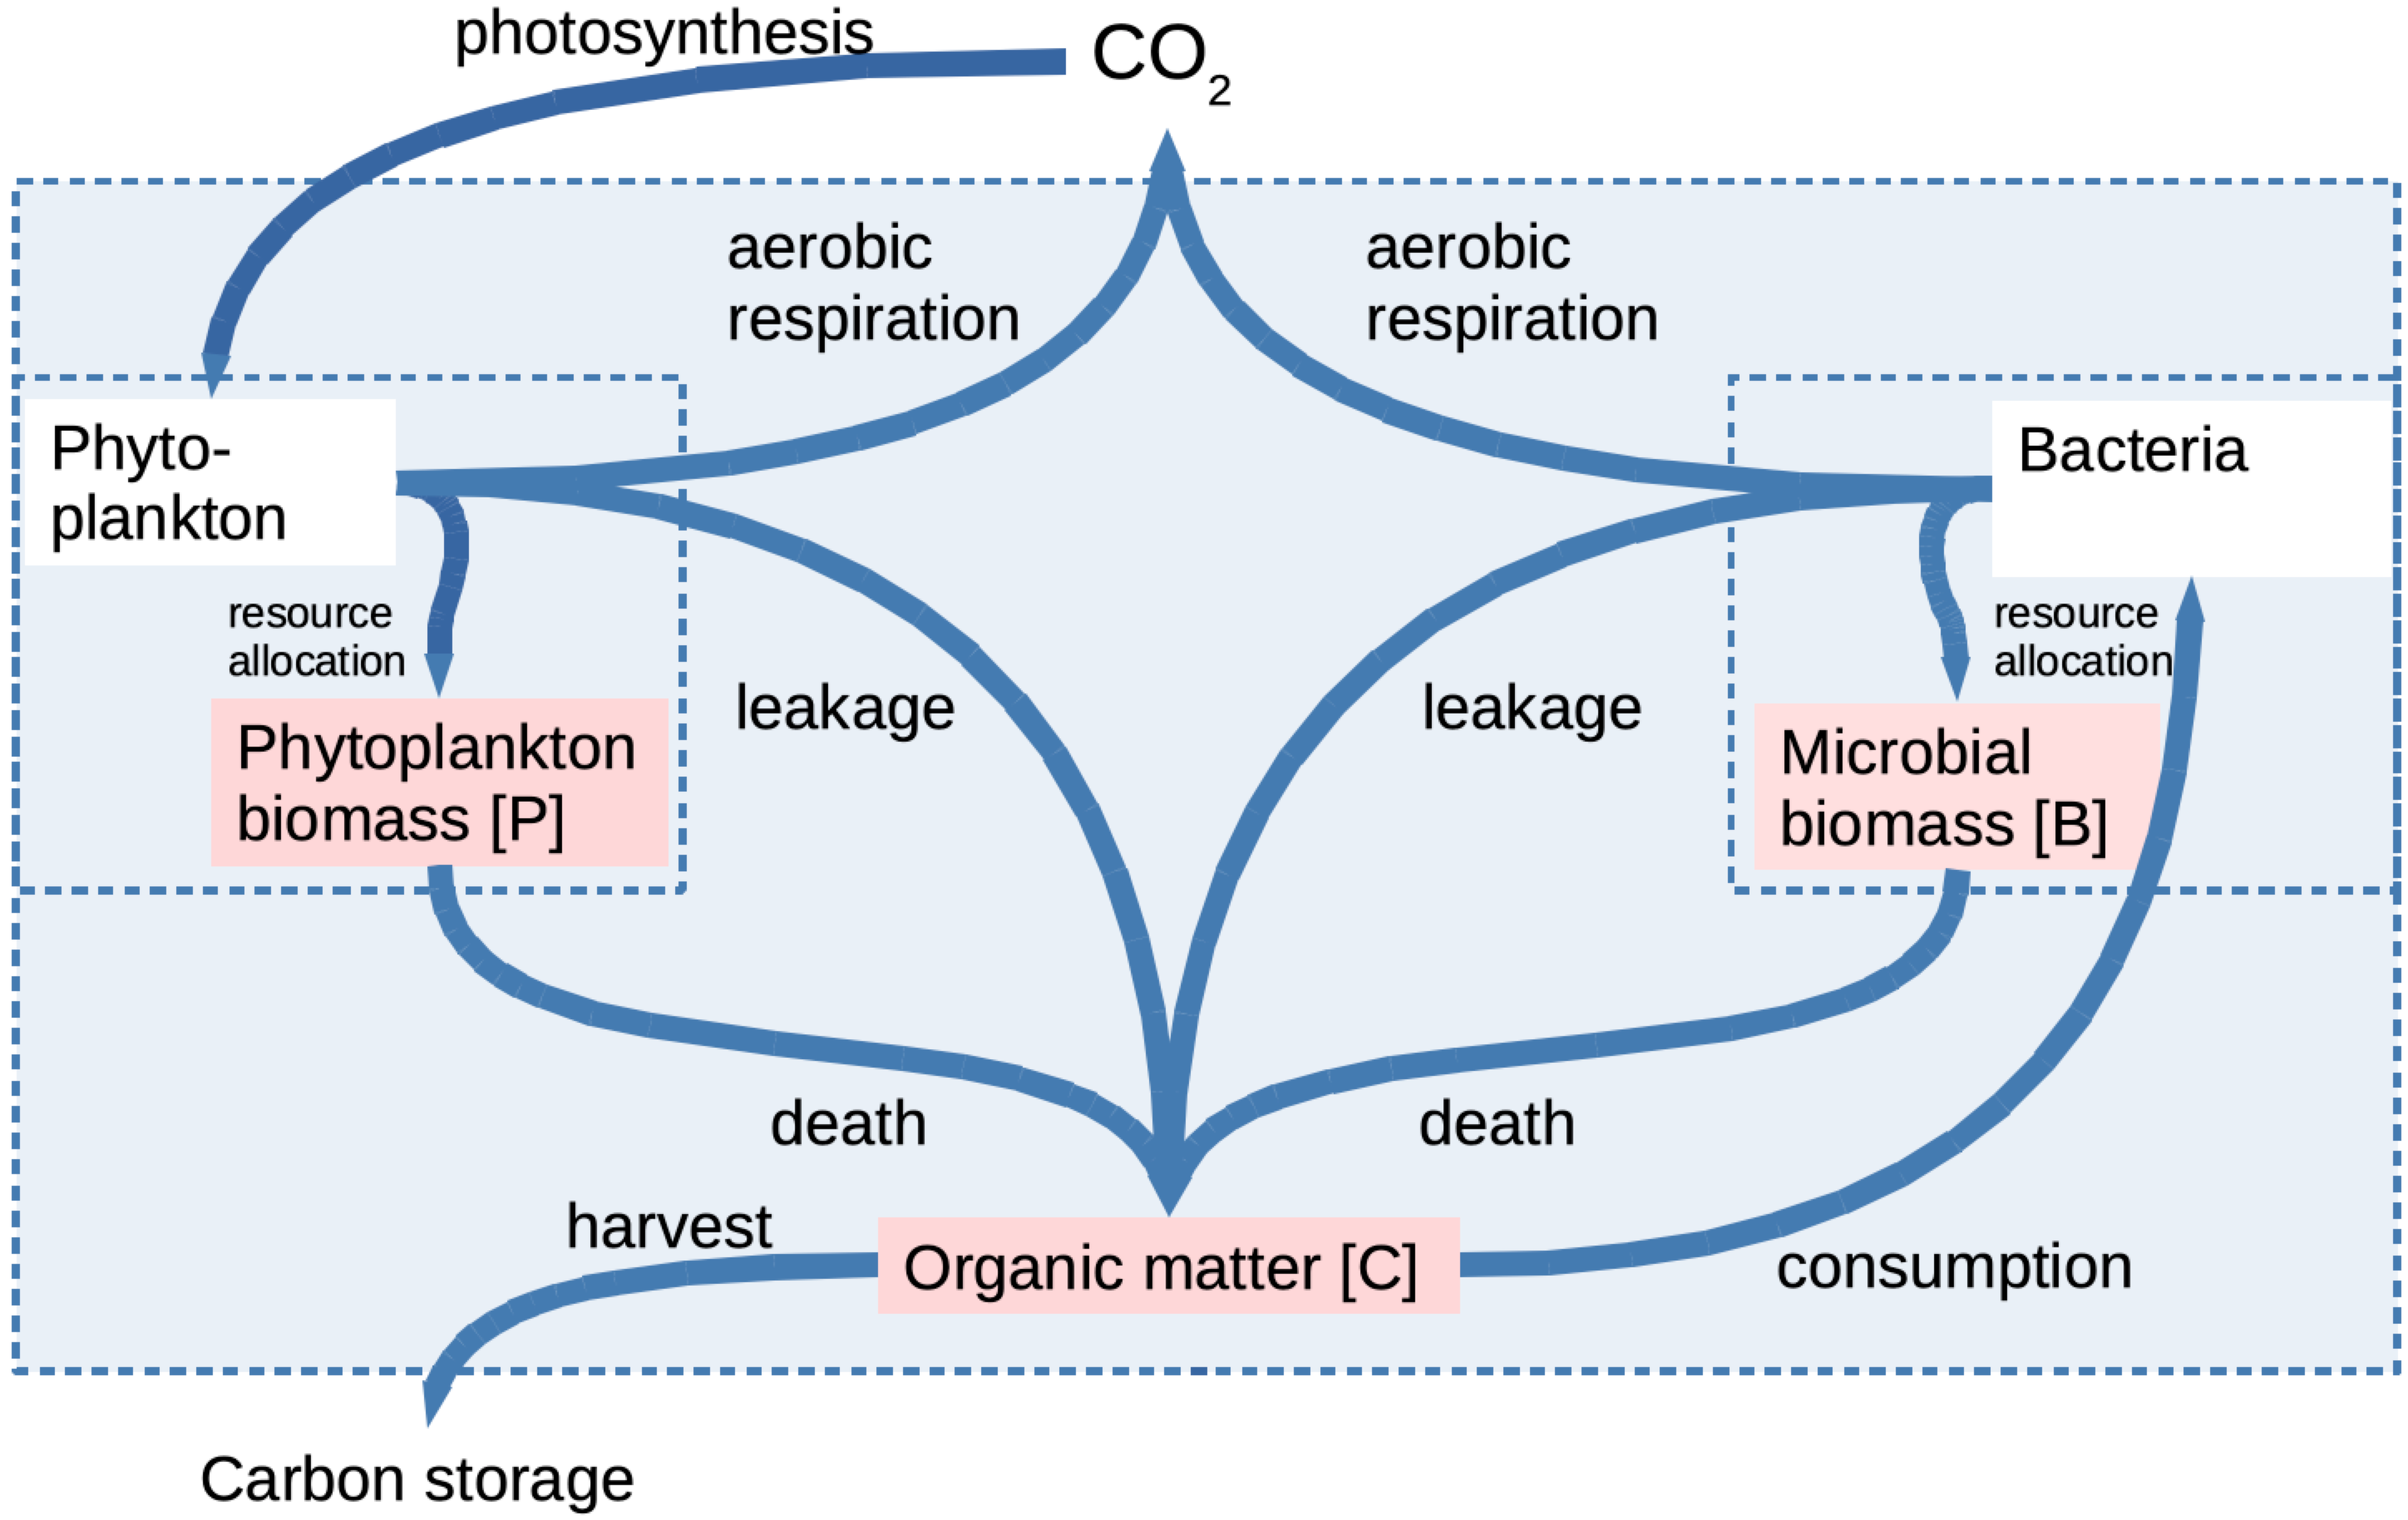
\includegraphics[width=.8\linewidth]{media/model.png}
    \caption[Model visualization]{Classification of dominant interactions in this project.  The two players shared all interactions with respective carbon pools but one, which was the energy acquiring method.}
    \label{modelInWord}
\end{figure}

\subsection{biological variables and parameter hyperspace}
Nine parameters were used, two sets of four biological parameters for the players P and B plus one carbon harvest rate parameter.  The harvest rate was sampled under a uniform prior ranged from 0 to 1 $day^{-1}$.  Due to data limitations, time unit was ``day" and biological parameters were divided into two categories for practicality: fractions and rates.

Fractions consisted of four dimensionless members, $\ePR$, $\eP$, $\eBR$ and $\eB$.  $\ePR$ and $\eBR$ were non-respired carbon fractions for P and B respectively.  $\eP$ and $\eB$ were carbon fractions incorporated into biomass for P and B respectively.

Rates consisted of four members with two similar units, which were $\gP$, $\mB$, $\aP$ and $\gB$.  $\gP$ was the specific growth rate for P and $\mB$ was the death rate for B.  They only linearly to its respective bio-engines.  $\aP$ was the intraspecific interference for P and $\gB$ was the resource clearance rate for B.  $\aP$ responded to the pairwise interactions within the P pool (hence $P^2$) while $\gB$ responded to the consumption of carbon from the finite C pool by B (hence $C\cdot B$).

Limited by available data, $\aP$, $\eBR$, $\eB$ and $\mB$ did not contain much data to work on.  Hence, parameter ranges for them were calculated by mean of available data $\pm$ the largest percentage range available in their respective category.  From the current data those two reference ranges were from $\ePR$ and $\gP$ respectively.  The resultant parameter space was then simulated by Latin Hypercube Sampling (LHS) technique under a uniform prior.  Detailed calculations for all parameters (including temperature standardisation procedures) were documented in the Appendix.

\begin{table}[H]
    \centering
    \caption[Algebra variables]{Table showing biological variables and corresponding ranges framing the parameter hyperspace}
    \begin{tabular}{cclll}\hline
        variable & unit & description & min (2dp) & max (2dp) \\\hline
        $N'(t)$ & $\dfrac{gC}{m^3\cdot day}$ & rate of change of respective carbon pool {\tiny($N=C,P,B$)} & - & - \\
        $N$ & $\dfrac{gC}{m^3}$ & carbon density for respective pool {\tiny($N=C,P,B$)} & - & - \\
        $\ePR$ & - & non-respired carbon fraction for P & 0.08 & 0.87 \\
        $\eP$ & - & assimilated carbon fraction for P & 0.4 & 1 \\
        $\gP$ & $day^{-1}$ & growth rate of P & 0.03 & 3.17 \\
        $\aP$ & $\dfrac{m^3}{gC\cdot day}$ & intraspecific interference of P & 0.02 & 1.52 \\
        $\eBR$ & - & non-respired carbon fraction for B & 0.13 & 1 \\
        $\eB$ & - & assimilated carbon fraction for B & 0.07 & 0.82 \\
        $\gB$ & $\dfrac{m^3}{gC\cdot day}$ & clearance rate of B & 0.10 & 3.50 \\
        $\mB$ & $day^{-1}$ & death rate of B & 0.01 & 0.63 \\
    \hline\end{tabular}
    \label{varInTab}
\end{table}

This parameter hyperspace was scanned for different value of harvest rates (denoted by $x$, unit day$^{-1}$).  Selected values of $x$ scanned were 0 to 10 with interval =0.1 for values lower than 1 and interval =1 onward.

\subsection{the model in equations}
Using the parameters defined in Table \ref{varInTab}, linkages in Fig.\ref{modelInWord} could be summarised in Eqn.\ref{eq:ode}.

\begin{equation}\left\{\begin{array}{rl}
    C'(t) &= \ePR(1-\eP)\cdot\gP\cdot P +\aP\cdot P^2 \underline{+(\eBR(1-\eB)-1)\cdot\gB\cdot C\cdot B +\mB\cdot B} \{-xC\}\\
    P'(t) &= \ePR\cdot\eP\cdot\gP\cdot P -\aP\cdot P^2\\
    \underline{B'(t)} &= \underline{\eBR\cdot\eB\cdot\gB\cdot C\cdot B -\mB\cdot B}
\end{array}\right.\label{eq:ode}\end{equation}

Considering different situation, the proposed model (Eq.\ref{eq:ode}) could be categorized into three components: the core, the bacterial (underlined) and the harvest (inside curly brackets) parts.

The core part resembled the approach of having a P-only system without continuous harvest of organic carbon.  Additional of the bacterial part resembled the P+B system without harvest.  The bacterial part was the B engine and its associated carbon pool.  Adding of the harvest part resembled the continuous organic carbon harvest from the respective pool in the system.  It is the only external forcing in the system representing an active perturbation of the natural ecological equilibrium.

The above proposed model hence was a full-geared with four skins: the ``P+B with harvest" (PBH, i.e. Eq.\ref{eq:ode}), ``P+B no harvest" (PBN), ``P-only with harvest" (PoH) and ``P-only no harvest" (PoN).

\subsection{solving the model}
Numerical solve through python3 (v3.7.3)\autocite{van1995python} SciPy (v1.2.3)\autocite{virtanen2020scipy} ``odeint" function showed a stable final stage in Eq.\ref{eq:ode} independent from initial values higher than $10^{-5}gC\cdot m^{-3}$ (or $10\mu gC\cdot m^{-3}$ ).  Since candidates for P and B were common organisms, boundary conditions from initial values were not considered biologically meaningful.  Hence analyses were based on the assumption of initial biomass densities of both P and B were above the boundary.

Analytical solve using SymPy (v1.5.1)\autocite{meurer2017sympy} revealed four alternative equilibria for PBH, two of them shared with PoH.  A single yet different equilibrium was found for PBN and PoN respectively (Table \ref{tab:eqm}).

\begin{table}[H]
    \centering
    \caption{Table of equilibria from the four variations of the proposed model (Eq.\ref{eq:ode})}
    \begin{tabular}{cl|ccc}\hline
        eqm & scenario & C & P & B (only if scenario contained B) \\\hline
        1 & PBH, PoH & 0 & 0 & 0 \\
        2 & PBH & $\dfrac{\mB}{\eBR\eB\gB}$ & 0 & $\dfrac{-x}{\gB(1-\eBR)}$ \\
        3 & PBH, PoH & $\dfrac{\eP(\ePR\gP)^2}{\aP x}$ & $\dfrac{\ePR\eP\gP}{\aP}$ & 0 \\
        4 & PBH & $\dfrac{\mB}{\eBR\eB\gB}$ & $\dfrac{\ePR\eP\gP}{\aP}$ & $\dfrac{(\ePR\gP)^2\eBR\eB\gB-\aP\mB x}{(1-\eBR)\aP\gB\mB}$ \\
        5 & PBN & C & 0 & 0 \\
        6 & PoN & - & P & - \\\hline
    \end{tabular}
    \label{tab:eqm}
\end{table}

In Table \ref{tab:eqm}, eqm 1, 2 were biologically meaningless. Eqm 1 indicated an empty aquarium was in a stable equilibrium.  Eqm 2 had an always-negative B biomass which was impossible.  Eqm 3 indicated that the PoH model could be interpreted by PBH when initial value of B was set zero.  Eqm 4 hinted for every pair of P and B in the system there would be a maximum value of $x$ (i.e. harvest rate).  The effect of $x$ would be investigated and discussed.  Eqm 5 and 6 were mathematically meaningless because they contained no parameters.  On a contrary, evaluating eqm 3 and 4 using $x=0$ gave out more logically-sounded and interpretable solutions.  Hence the scanning and analyses were based on these two analytical solutions.

\subsection{model simulation analysis}
11 evenly-distributed values within each parameter range (Table \ref{varInTab}) were selected with R(v4.0.2)\autocite{r2020r}.  5500 unique biological parameter value combinations were sampled using LHS technique under a uniform prior.  The expected frequency of each value of each parameter was 500.  The LHS sample pool was analytically scanned for all harvest rates (Table \ref{tab:eqm}).  A positive value for a carbon pool indicated the respective pool existed at stable equilibrium.  Hence the total carbon ($C+P+B$ carbon pools) value was only considered biologically valid if all component carbon pools have a positive value.
%% analyses
Wilcox signed-rank test (W-test) was carried out between the natural log values of total carbon and yield flux ($x\times C$).  Yields for ``no harvest" situations were set equal to the total carbon of such systems.  Total carbon and yield flux were also compared based on individual biological parameters, categorised by the carbon removal rate ($x$).

\end{document}
